\documentclass[a4paper,11pt]{article}
\usepackage[left=3cm,top=3cm,right=2cm,bottom=2cm]{geometry}
\usepackage[brazilian, english]{babel}
\usepackage[utf8]{inputenc}
\usepackage[numbers]{natbib}
\usepackage{mathtools}
\usepackage{amssymb}
\usepackage{amsmath}
\usepackage{epigraph}
\usepackage{indentfirst}
\usepackage{graphicx}
\usepackage{wrapfig}
\usepackage{setspace}
\usepackage[hidelinks]{hyperref}
\usepackage{xcolor}
\usepackage{adjustbox}
\usepackage{minted}
\newcommand{\tabitem}{~~\llap{\textbullet}~~}
\newcommand*{\SignatureAndDate}[4]{%
	\parbox{7cm}{
      \centering
      \rule{6cm}{1pt}\\
       #1
       
       #2
    }
    \hfill
\parbox{7cm}{
      \centering
      \rule{6cm}{1pt}\\
       #3
       
       #4
    }
}%
\usepackage{float}

\floatstyle{ruled}
\newfloat{program}{thp}{lop}
\floatname{program}{Program}

\onehalfspacing

\title{Relatório}

\renewcommand{\familydefault}{\sfdefault}

\begin{document}
\selectlanguage{brazilian}

%%% CAPA %%%

\begin{titlepage}

\begin{wrapfigure}[2]{l}{0.2\textwidth}
	\label{Logo UFABC}
	\vspace{-1\baselineskip}
	\centering
	\includegraphics[width=0.25\textwidth]{images/Logo_UFABC}
\end{wrapfigure}

\uppercase{Universidade Federal do ABC}

\uppercase{Bacharelado em Ciência da Computação}

\vfill
\begin{center}

\uppercase{\textbf{Implementação de uma calculadora em FPGA}}

\vfill

\uppercase{Gustavo Henrique Barrionuevo (11017011)\\ Nilton Gomes Martins Junior (11029213)}
\vspace{1cm}

Orientador: Prof. Dr. Rodrigo Moreira Bacurau

\vfill

Santo André -- SP

2019
\end{center}
\end{titlepage}

%%% FIM DA CAPA %%%

%%% FOLHA DE ROSTO %%%

\begin{titlepage}
\begin{center}
\uppercase{\textbf{Gustavo Henrique Barrionuevo \\ Nilton Gomes Martins Junior}}

\vfill

\uppercase{\textbf{Implementação de uma calculadora em FPGA}}
\end{center}

\vfill

\hfill \begin{minipage}{0.5\textwidth}
Relatório apresentado ao curso Bacharelado em Ciência da Computação da Universidade Federal do ABC como requisito parcial para aprovação na disciplina de Sistemas Digitais.
\vspace{1cm}

Orientador: Prof. Dr. Rodrigo Moreira Bacurau
\end{minipage}

\vfill

\begin{center}
Santo André -- SP

2019
\end{center}
\end{titlepage}

%%% FIM DA FOLHA DE ROSTO %%%
\selectlanguage{brazilian} 

%%% SUMÁRIO %%%
\newpage
\tableofcontents

\newpage
\section{Introdução}

Este trabalho implementa uma calculadora aritmética simples em \textit{VHDL}, com o projeto baseado sobre a placa de desenvolvimento \textit{ALTERA Development and Education 1}, com o \textit{FPGA Cyclone II EP2C20F484C7}.

Esta calculadora é capaz de realizar operações aritméticas fundamentais (soma, subtração, multiplicação e divisão). As operações ocorrem em sequência, então as precedências são definidas unicamente com base na ordem com que as operações e os operandos são definidos.

Os operandos são números inteiros, representados internamente na forma de complemento de dois.

A visualização dos operandos e do resultado é feita por meio de um conjunto de quatro \textit{displays} de sete segmentos.

Esta calculadora recebe os valores de entrada e as operações, bem como quaisquer outros comandos, através de um teclado com interface \textit{PS2} conectado diretamente à placa de desenvolvimento.

Além das operações aritméticas, também foi implementado o controle de brilho dos \textit{displays} de sete segmentos, através de um controlador do tipo \textit{PWM} (\textit{Pulse Width Modulation}).

\newpage
\section{Manual de utilização}

A calculadora foi implementada no \textit{FPGA Cyclone II EP2C20F484C7}, de maneira que o uso da mesma fica limitado à dispositivos compatíveis com essa arquitetura. Este manual supõe que o leitor está utilizando o projeto na placa \textit{ALTERA Development and Education 1} (Figura \ref{fig:altera_de1}).

\begin{figure}[H]
\makebox[\textwidth][c]
{\includegraphics[width=0.6\textwidth]{images/altera_de1.jpg}}
\caption{Placa de desenvolvimento \textit{ALTERA Development and Education 1}.}
\label{fig:altera_de1}
\end{figure}

\subsection{Carregamento do programa e preparação do \textit{kit}}

O carregamento do arquivo de saída no formato \mintinline{shell}{.sof} é feito através do \textit{software ALTERA QUARTUS}. O procedimento a ser seguido para a realização do carregamento é descrito em detalhes por Rodrigo M. Bacurau \cite{bacurau_intro}.

Como a entrada de dados para as operações aritméticas é feita exclusivamente com o teclado, é necessário conectar um teclado com padrão \textit{PS2} na entrada apropriada da placa de desenvolvimento.

\subsection{Operações aritméticas com dois operandos}

Com o código carregado na placa e o teclado devidamente conectado, o programa encontra-se no estado inicial, onde nenhum operando e nenhuma operação foram definidos, e o resultado padrão é 0.

A calculadora suporta entrada de números representáveis com até 13 \textit{bits} em complemento de dois, isso é, podem ser inseridos números com módulo no intervalo de 0 à 4095. Os valores negativos são obtidos indiretamente, através de operações de subtração ou de multiplicação (caso o resultado atual seja negativo). O intervalo de valores que podem ser representados na calculadora é [-4096, 4095]. Não é possível inserir valores maiores do que esse (há um bloqueio de leitura). Se alguma operação for realizada de tal forma que o resultado não pertença ao intervalo, o resultado será \textit{ERRO}.

Ao se digitar uma entrada válida com o teclado, o que pode ser feito tanto com o teclado numérico (\textit{numpad}), quanto com as teclas numéricas comuns, o valor de entrada é exibido nos \textit{displays} de sete segmentos, substituindo o resultado anterior.

Com a inserção de um operando finalizada, é necessário selecionar o operador, utilizando o teclado numérico. As opções são:

\begin{itemize}
	\item +: adição;
	\item -: subtração;
	\item *: multiplicação;
	\item /: divisão (inteira).
\end{itemize}

Nesta etapa, se for selecionada alguma operação por engano, basta pressionar a tecla correspondente à operação desejada para que a operação seja sobrescrita, não sendo necessário reiniciar o cálculo com a inserção do primeiro operando.

Após a seleção da operação desejada, prossegue-se com a definição do segundo operando, que é feita da mesma maneira com que o primeiro foi definido, observando as mesmas restrições. 

Uma vez que o operando tenha sido selecionado, basta apertar a tecla \textit{ENTER} para que o resultado da operação seja exibido nos \textit{displays}. Para números positivos dentro do intervalo válido de operação a visualização é convencional, com o algarismo mais significativo do lado esquerdo. Para números negativos a representação do sinal se dá de duas possíveis maneiras:

\begin{itemize}
	\item Sinal representado num \textit{display} e com LED vermelho: Caso o resultado negativo tenha módulo inferior à 1000, isto é, está contido no intervalo [-999, -1], o LED vermelho número 9 (LEDR9, localizado mais à esquerda da placa) será aceso e o sinal será exibido no \textit{display} da esquerda do algarismo mais significativo. Por exemplo, o número -1 tem seu sinal representado no terceiro \textit{display}, da esquerda para a direita, enquanto o número -100 tem o sinal no primeiro \textit{display}. Se houverem \textit{displays} à esquerda do sinal, os mesmos permanecerão desativados;
	
	\item Sinal representado apenas com LED vermelho: Caso o sinal não possa ser representado nos \textit{displays}, quando o resultado tem módulo superior ou igual à 1000 e, portanto, demanda quatro algarismos, apenas o LED vermelho ficará aceso.
\end{itemize}

\subsection{Operações aritméticas em sequência}

Com um resultado salvo, é possível operar sobre o mesmo utilizando uma recorrência com a última operação e o último operando. Isto é realizado através de sucessivos pressionamentos da tecla \textit{ENTER}. Por exemplo, supondo que utiliza-se o estado inicial, com resultado 0, e deseja-se incrementar este resultado em 2 unidades à cada pressionamento de \textit{ENTER}, basta selecionar a operação de adição (tecla +), e o operando 2. Ao se apertar \textit{ENTER} pela primeira vez, conforme uma operação convencional, o resultado exibido será 2 (uma vez que 0 + 2 = 2). Ao se pressionar \textit{ENTER} novamente, sem a necessidade de se selecionar uma operação ou outro operando, o valor 2 será novamente adicionado ao resultado atual, 2, e o resultado 4 será exibido (2 + 2 = 4). Isso pode ser realizado indefinidamente, respeitando a limitação de representação no intervalo [-4096, 4095].

As operações em sequência também pode ser feitas com outras operações e operandos. Após cada operação ser finalizada, se um resultado válido for obtido, este resultado é armazenado e utilizado como o primeiro operando da operação subsequente. Assim, basta selecionar uma nova operação e outro número e apertar \textit{ENTER} novamente para reutilizar o resultado anterior num novo cálculo.

\subsection{Limpando a memória da calculadora}

Tanto o cancelamento de qualquer operação quanto a saída do estado de \textit{ERRO} são feitos através da tecla \textit{ESC}. Com isso todos os resultados são limpos da memória e a calculadora é zerada, retornando ao estado inicial.

\subsection{Controle de brilho do \textit{display}}

O controle de brilho do \textit{display} é feito através das oito primeiras chaves (\textit{SW0-SW7}) . Com todas as chaves em nível baixo (posição inferior) se obtém o brilho máximo. Com os oito \textit{bits} representados por cada chave, o brilho pode variar entre 256 níveis de intensidade. A chave com o \textit{bit} mais significativo é a SW7.

O controle de brilho dos \textit{displays} é feita independentemente da operação da calculadora. Desse modo, o controle de brilho com as chaves pode ser feito à qualquer momento sem nenhum impacto ao estado atual da operação aritmética corrente.

\newpage
\section{Organização do projeto} \label{sec: org}

O projeto é estruturado em torno do arquivo principal \mintinline{shell}{calculator.vhd}, que contém a descrição da máquina de estados que é o cerne deste trabalho. 

O código é descrito no apêndice \ref{sec:apend_principal}.

A máquina de estados é descrita de forma geral pela Figura \ref{fig:fsm}.

\begin{figure}[!htb]
\makebox[\textwidth][c]
{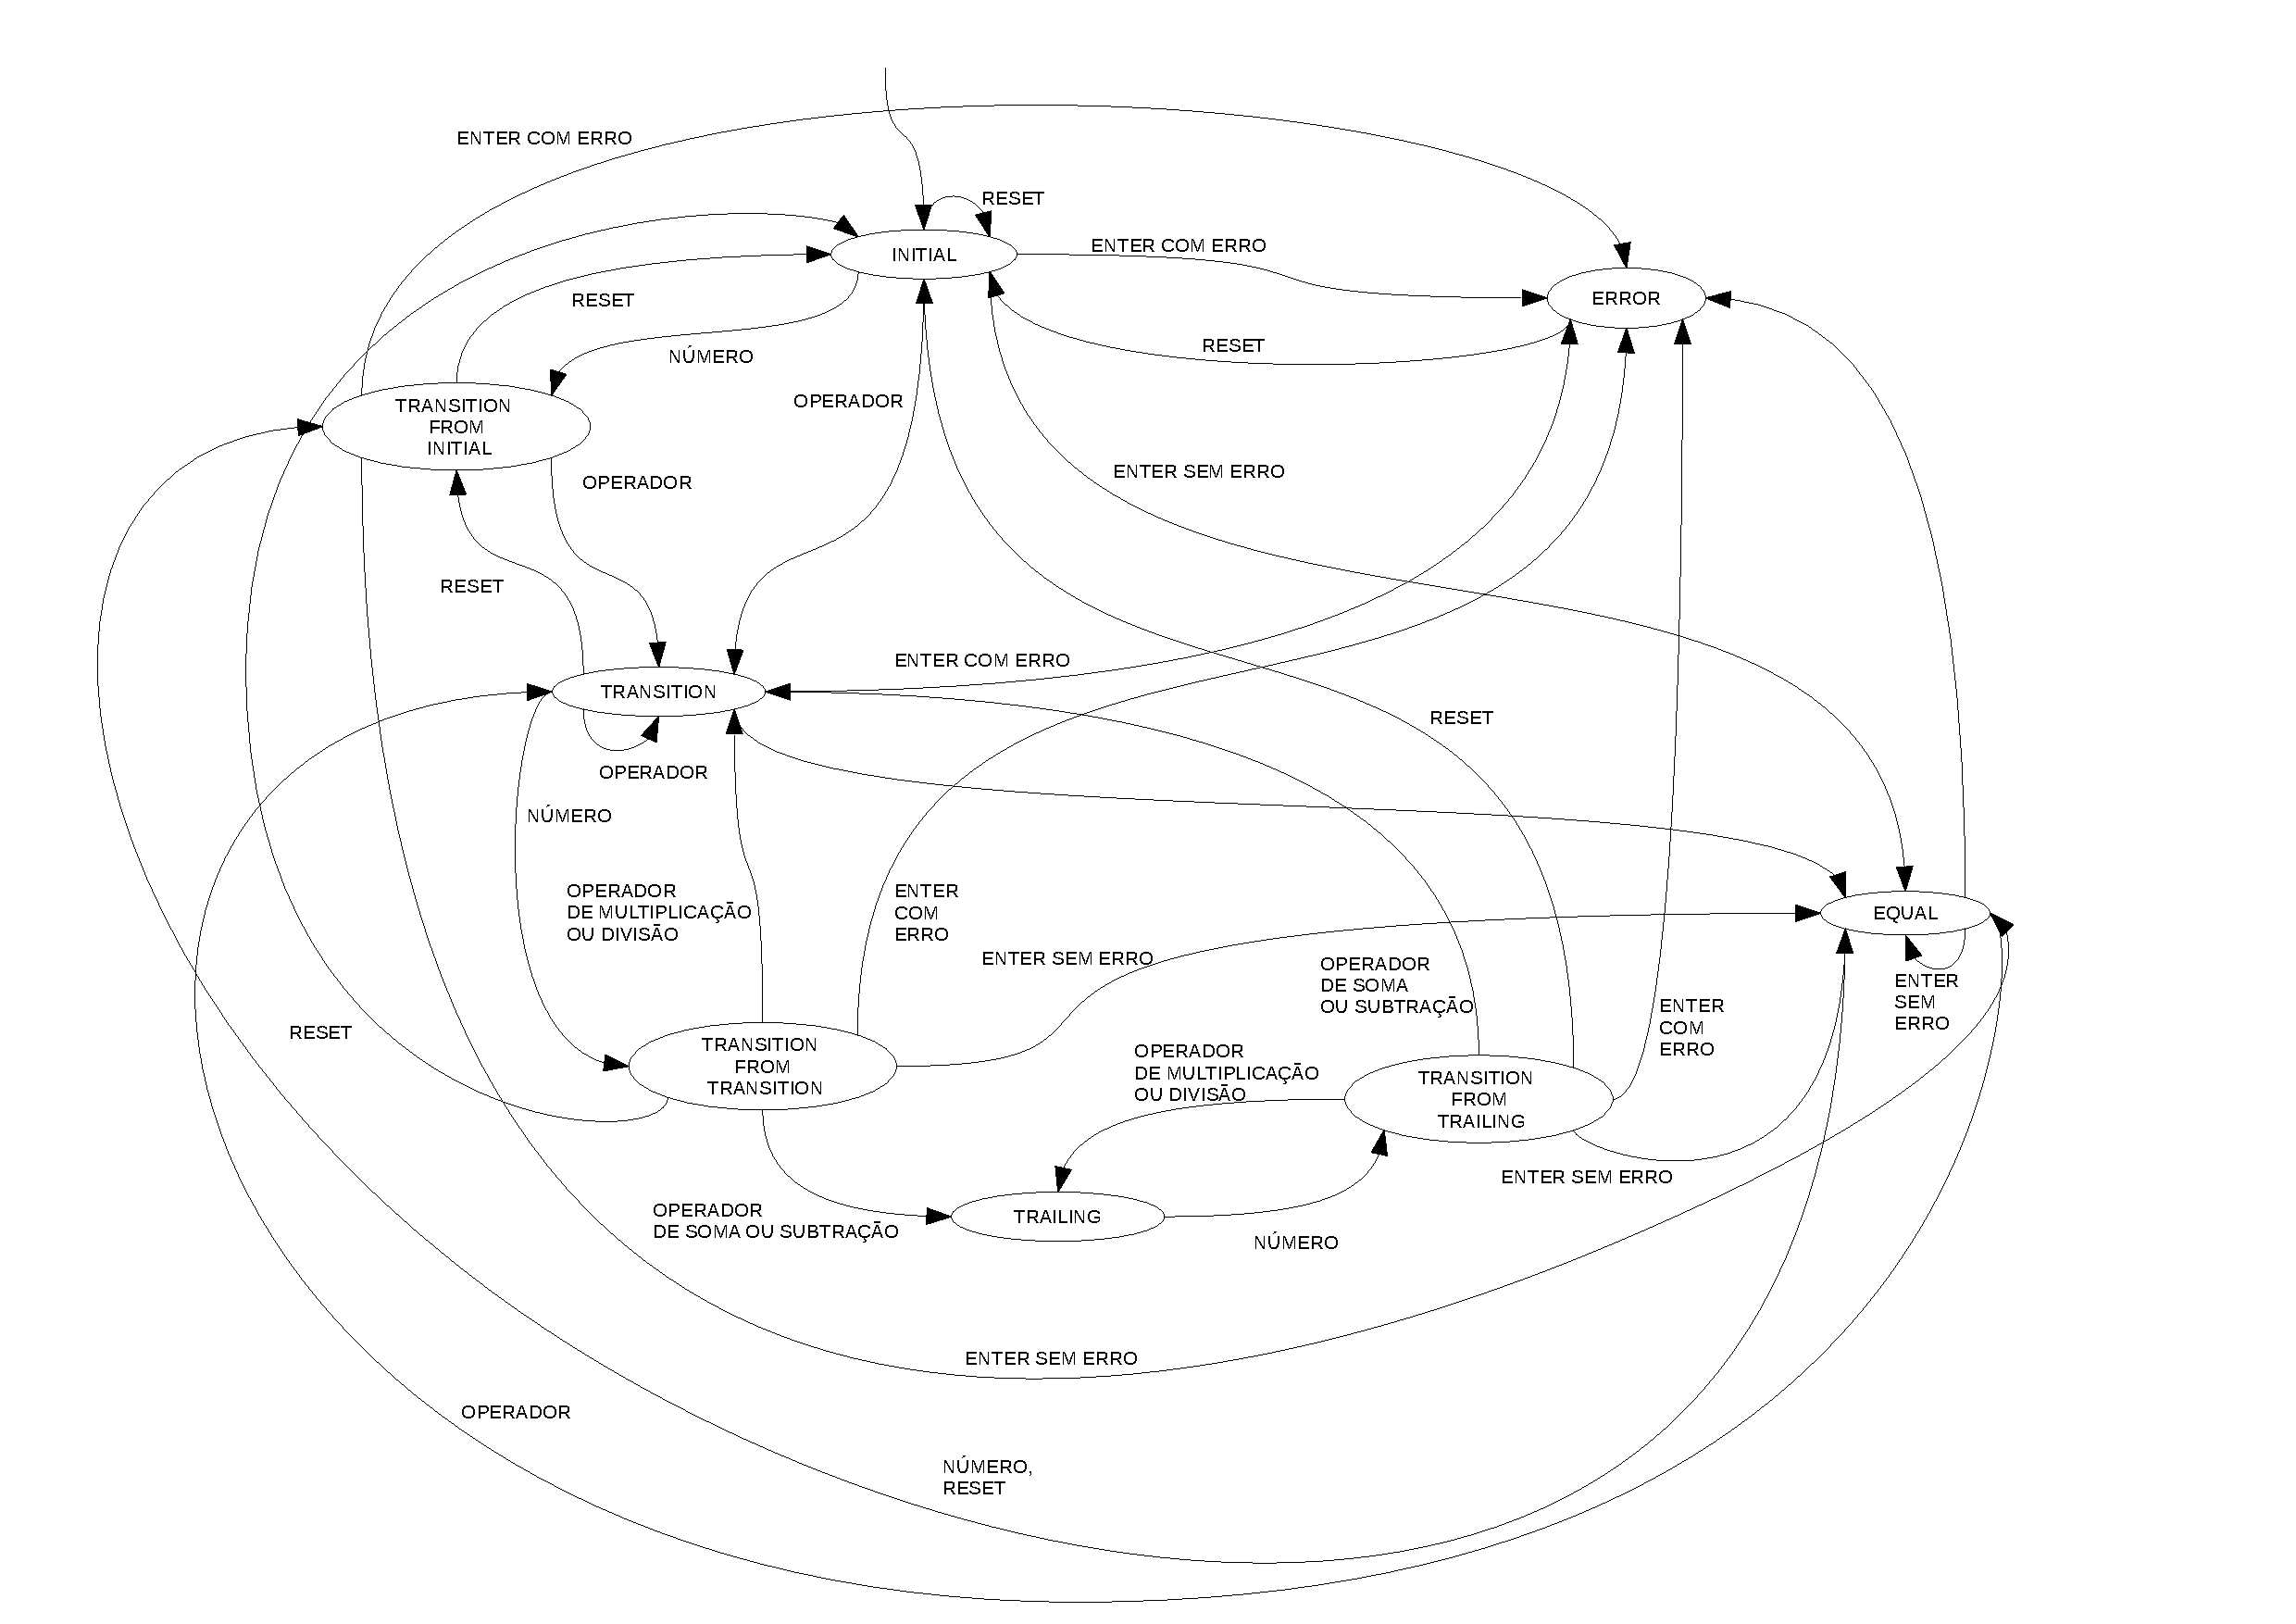
\includegraphics[width=1\textwidth]{images/fsm.pdf}}
\caption{Descrição geral da máquina de estados.}
\label{fig:fsm}
\end{figure}

Existem três operandos de interesse: o primeiro, o segundo e o subsequente, denominados no código como \mintinline{shell}{fn}, \mintinline{shell}{sn} e \mintinline{shell}{tn}, respectivamente. Os dois primeiros definem as operações convencionais e o terceiro é utilizado como uma variável auxiliar para operações sequenciais.

Os estados são descritos por:

\begin{itemize}
	\item \textit{INITIAL}: Estado inicial, com resultado zero. Obtido no início da execução ou com o uso do \textit{RESET};
	\item \textit{TRANSITION FROM INITIAL}: Estado que identifica a entrada do primeiro operando;
	\item \textit{TRANSITION}: Estado que identifica que o primeiro operando foi definido e determina a entrada da operação;
	\item \textit{TRANSITION FROM TRANSITION}: Identifica a entrada do segundo operando, após a definição da operação;
	\item \textit{EQUAL}: Após a inserção do segundo operando, exibe o resultado da operação, caso o mesmo seja válido;
	\item \textit{TRAILING}: Caso onde são feitas operações sequenciais, lê-se um operador para a próxima operação sobre o resultado atual;
	\item \textit{TRANSITION FROM TRAILING }: Ainda no caso de operações sequenciais, lê o número subsequente, que se torna o segundo operando, enquanto que o primeiro operando é o resultado da operação anterior;
	\item \textit{ERROR}: Estado de erro, quando algum resultado inválido é obtido (fora do intervalo pré-determinado ou divisão por zero).
\end{itemize}

Além da definição dos estados e transições, o arquivo principal também estrutura a interação entre as bibliotecas genéricas (\mintinline{shell}{general}), de entrada e saída (\mintinline{shell}{io}) e numérica (\mintinline{shell}{numeric}). Os arquivos que constituem cada uma destas bibliotecas estão dentro do diretório \mintinline{shell}{/lib/}.

\subsection{Biblioteca genérica}

A biblioteca genérica é composta pelos seguintes arquivos:

\begin{itemize}
	\item \mintinline{shell}{binary_to_bcd.vhd}: realiza a conversão de um valor binário de 13 \textit{bits} (em complemento de 2) para o formato \textit{BCD} com 16 \textit{bits}.
	
	O código está descrito na seção \ref{sec:apend_bin_bcd}.
	
	Este código, implementado em outra aula prática da disciplina de Sistemas Digitais \cite{bacurau_pwm_dd}, é uma replicação do algoritmo de \textit{Double-Dabble}, que codifica um número binário representado por uma quantidade arbitrária de \textit{bits} na forma \textit{BCD}. O algoritmo é um registrador de deslocamento que itera tantas vezes quantos forem o número de \textit{bits} e, a cada iteração, adiciona o valor 3 à cada \textit{nibble} se este representar um valor numérico superior à 4;
	
	\item \mintinline{shell}{conv_7seg.vhd}: converte um valor binário de 4 \textit{bits} referente à um dígito de 0 à 9, sinal negativo ou valor nulo, para \textit{display} de sete segmentos.
	
	O código é descrito na seção \ref{sec:apend_bin_7seg};
	
	\item \mintinline{shell}{general.vhd}: define o pacote com os demais arquivos da biblioteca genérica;

	\item \mintinline{shell}{pwm.vhd}: define o controlador \textit{PWM} para o controle de brilho dos \textit{displays} de sete segmentos.
	
	O código é descrito em \ref{sec:apend_pwm}.
	
	O algoritmo consiste numa combinação de um contador e um comparador. O contador incrementa a contagem a cada pulso de \textit{clock} e o comparador ativa a saída caso a contagem seja inferior ao valor do \textit{duty-cycle}. O tempo que a saída permanece ativa em relação ao período da onda determina a potência luminosa dos \textit{LEDs} de cada \textit{display} de sete segmentos;
	
	\item \mintinline{shell}{scancode_to_calc_input.vhd}: realiza a conversão de uma entrada do teclado \textit{PS2} para um vetor de 5 \textit{bits} representando um dígito, uma operação aritmética, o comando \textit{ENTER} ou o comando \textit{CLEAR}.
	
	O código é descrito na seção \ref{sec:apend_scancode}.
\end{itemize}

\subsection{Biblioteca de I/O}

A biblioteca de entrada e saída é composta pelos seguintes arquivos:

\begin{itemize}
	\item \mintinline{shell}{io.vhd}: define o pacote com os demais arquivos da biblioteca de entrada e saída;
	\item \mintinline{shell}{kbdex_ctrl.vhd}: define o controlador para o teclado \textit{PS2}, permitindo a leitura do código referente à um conjunto de até três teclas, totalizando 48 \textit{bits};
	\item \mintinline{shell}{ps2_iobase.vhd}: realiza a comunicação com o teclado através da porta \textit{PS2}.
\end{itemize}

\subsection{Biblioteca numérica}

A biblioteca numérica contem um único arquivo, \mintinline{shell}{numeric.vhd}, que define o pacote contendo todas as operações aritméticas, bem como os algoritmos que as implementam.

O código com o pacote é descrito em \ref{sec:apend_numeric}

O pacote com as operações aritméticas contém as funções:

\begin{itemize}
	\item \mintinline{vhdl}{bit_adder_subtractor()}: Realiza as operações de soma e subtração com apenas um \textit{bit}. É o algoritmo de um somador completo;
	
	\item \mintinline{vhdl}{ripple_adder_subtractor()}: Realiza as operações de soma e subtração com vetores de \textit{bits}. Este algoritmo implementa a estrutura de um somador completo de múltiplos \textit{bits}, que é o encadeamento de somadores completos de um \textit{bit} em cascata, onde o \textit{carry-out} de um é alimentado ao \textit{carry-in} do seguinte (mais significativo);
	
	\item \mintinline{vhdl}{booth_multiplier()}: Implementa um multiplicador de Booth para vetores de \textit{bits} representando números em complemento de dois. O algoritmo do multiplicador de Booth é baseado numa implementação descrita em aula \cite{bacurau_booth};
	
	\item \mintinline{vhdl}{divide()}: Utiliza o método de divisão do pacote \mintinline{vhdl}{IEEE.NUMERIC_STD}.
	
\end{itemize}

\newpage
\section{Problemas identificados e não resolvidos e demais limitações de projeto}

Não foram detectados \textit{bugs} com solução pendente, mas listam-se as principais limitações do projeto:

\begin{itemize}
	\item Há a limitação de representação com 13 \textit{bits}, de modo que os valores inseridos e/ou resultados obtidos devem estar contidos no intervalo [-4096, 4095];
	\item Os valores podem ser representados com os quatro \textit{displays}, mas o sinal negativo para números com quatro dígitos precisou ser representado exclusivamente através de um LED auxiliar;
	\item Todos os valores de entrada e resultados são inteiros, não foi implementado ponto fixo ou flutuante;
	\item Muito embora todas as operações aritméticas básicas tenham sido implementadas, a divisão é inteira, e o resto é desconsiderado, isto é, o resultado da divisão entre dois operandos $a, b \in \mathbb{Z}$ é dado por $a \div b = \lfloor a/b \rfloor$.
\end{itemize}

\newpage
\section{Autoria dos códigos utilizados}

Para a estrutura da aplicação descrita na Seção \ref{sec: org}, são feitas as considerações referentes à autoria dos códigos implementados.

São códigos originais aqueles contidos nos arquivos;

\begin{itemize}
	\item \mintinline{shell}{binary_to_bcd.vhd};
	\item \mintinline{shell}{conv_7seg.vhd};
	\item \mintinline{shell}{general.vhd};
	\item \mintinline{shell}{pwm.vhd};
	\item \mintinline{shell}{scancode_to_calc_input.vhd};
	\item \mintinline{shell}{io.vhd};
\end{itemize}

O trecho de código do arquivo principal, \mintinline{shell}{calculator.vhd}, que estrutura a máquina de estados em \textit{VHDL} é baseado em uma implementação em \textit{Javascript} por Robert Vunabadi \cite{vunabandi}. O resto do código contido no arquivo implementa as bibliotecas númerica, de entrada e saída e outras generalidades. Esta parte do código é original.

Para os códigos da biblioteca númerica, o somador/subtrator completo de um \textit{bit} e o somador/subtrator completo em cascata foram implementados originalmente em aulas práticas anteriores da disciplina \cite{bacurau_somador}. 

Os códigos da biblioteca de entrada e saída referentes à comunicação com o teclado \textit{PS2} foram elaborados por Thiago Borges Abdnur, do Instituto de Computação da Unicamp (Universidade Estadual de Campinas) \cite{abdnur}. No contexto de entrada e saída, apenas o código que realiza a conversão do \textit{scancode} do teclado para um formato internamente interpretável é original (este código está contido na biblioteca genérica).

\newpage

\bibliography{doc}
\bibliographystyle{plainnat}

\newpage
\appendix
\section{Apêndice - Códigos desenvolvidos} \label{sec:apend_a}

Os códigos desenvolvidos e implementados são brevemente discutidos.

\subsection{Código principal} \label{sec:apend_principal}

O arquivo \mintinline{shell}{calculator.vhd} contém a descrição da máquina de estados que define o funcionamento da calculadora. O código é exibido à seguir.

\begin{minted}
[
frame=lines,
framesep=2mm,
baselinestretch=1.2,
fontsize=\footnotesize,
breaklines,
linenos
]
{vhdl}
LIBRARY ieee;
USE ieee.std_logic_1164.ALL;

LIBRARY lib;
USE lib.io.ALL;
USE lib.general.ALL;
USE lib.numeric.ALL;

ENTITY calculator IS
PORT
(
------------------------	Clock Input	 	------------------------
clock_24 : 	IN	STD_LOGIC_VECTOR (1 DOWNTO 0);	--	24 MHz
clock_27 :	IN	STD_LOGIC_VECTOR (1 DOWNTO 0);	--	27 MHz
clock_50 : 	IN	STD_LOGIC;						--	50 MHz

------------------------	Push Button		------------------------
key :	IN	STD_LOGIC_VECTOR (3 DOWNTO 0);	--	Pushbutton[3:0]

------------------------	DPDT Switch		------------------------
sw 	:	IN	STD_LOGIC_VECTOR (9 DOWNTO 0);	--	Toggle Switch[9:0]

------------------------	7-SEG Display	------------------------
hex0 	:	OUT	STD_LOGIC_VECTOR (6 DOWNTO 0);	--	Seven Segment Digit 0
hex1 	:	OUT	STD_LOGIC_VECTOR (6 DOWNTO 0);	--	Seven Segment Digit 1
hex2 	:	OUT	STD_LOGIC_VECTOR (6 DOWNTO 0);	--	Seven Segment Digit 2
hex3 	:	OUT	STD_LOGIC_VECTOR (6 DOWNTO 0);	--	Seven Segment Digit 3

----------------------------	LED		----------------------------
ledg 	:	OUT	STD_LOGIC_VECTOR (7 DOWNTO 0);	--	LED Green[7:0]
ledr 	:	OUT	STD_LOGIC_VECTOR (9 DOWNTO 0);	--	LED Red[9:0]

------------------------	PS2		--------------------------------
ps2_dat	:	INOUT	STD_LOGIC;	--	PS2 Data
ps2_clk	:	INOUT	STD_LOGIC	--	PS2 Clock
);
END calculator;

ARCHITECTURE struct OF calculator IS

SIGNAL clockhz, resetn 	: STD_LOGIC;
SIGNAL key0 				: STD_LOGIC_VECTOR(15 DOWNTO 0);
SIGNAL lights, key_on	: STD_LOGIC_VECTOR(2 DOWNTO 0);

-- Sinal utilizado para armazenar os possíveis
-- valores de entrada do teclado PS2.
SIGNAL calc_input : STD_LOGIC_VECTOR(4 DOWNTO 0);

-- Sinal utilizado para armazenar o código BCD
-- que será utilizado para apresentar os valores
-- númericos da calculadora nos displays de 7 segmentos
SIGNAL bcd : STD_LOGIC_VECTOR(15 DOWNTO 0);

-- Sinal utilizado para armazenar o primeiro operando da
-- calculadora
SIGNAL first_number : STD_LOGIC_VECTOR(N-1 DOWNTO 0);
-- Sinal utilizado para armazenar o segundo operando da
-- calculadora
SIGNAL second_number : STD_LOGIC_VECTOR(N-1 DOWNTO 0);
-- Sinal utilizado para armazenar o operando de trailing da
-- calculadora
SIGNAL trailing_number : STD_LOGIC_VECTOR(N-1 DOWNTO 0);

-- Sinal utilizado para armazenar o valor atual do display
SIGNAL display_number : STD_LOGIC_VECTOR(N-1 DOWNTO 0);

-- Sinal utilizado para armazenar o primeiro operador da
-- FSM da calculadora
SIGNAL operation1 : STD_LOGIC_VECTOR(4 DOWNTO 0);

-- Sinal utilizado para armazenar o segundo operador da
-- FSM da calculadora
SIGNAL operation2 : STD_LOGIC_VECTOR(4 DOWNTO 0);

-- Definição dos 8 possíveis estados da máquina de
-- estados da calculadora.
TYPE state_type IS (
INITIAL,
TRANSITION_FROM_INITIAL,
TRANSITION,
TRANSITION_FROM_TRANSITION,
TRAILING,
TRANSITION_FROM_TRAILING,
EQUAL,
ERROR
);

-- Sinais utilizados para armazenar o estado atual (state)
-- e o próximo estado (next_state) da máquina de estados
-- da calculadora.
SIGNAL state, next_state : state_type;

SIGNAL pwm_out : STD_LOGIC;

SIGNAL duty : STD_LOGIC_VECTOR(7 DOWNTO 0);

-- Sinais utilizados para armazenar os valores
-- dos quatro displays de 7 segmentos
SIGNAL f0, f1, f2, f3 : STD_LOGIC_VECTOR(6 DOWNTO 0);

-- Sinal utilizado para indicar a ocorrência de algum
-- erro na ultima operação realizada pela calculadora.
SIGNAL error_result : STD_LOGIC;

BEGIN

resetn <= key(0);

-- Definição do duty utilizado pelo gerador PWM.
duty <= sw(7 DOWNTO 0);

-- Instanciação do controlador PWM.
pwm_controller: pwm PORT MAP(
clk => clock_50,
enable => '1',
rstn => '1',
duty => duty,
pwm_out => pwm_out
);

-- Responsável pela conversão dos scancodes do teclado para um formato
-- interno utilizado na calculadora.
conv_input: scancode_to_calc_input PORT MAP(
scancode => key0(7 DOWNTO 0),
calc_input => calc_input
);

-- Processo responsável pelo controle de brilho dos displays de 7 segmentos.
-- Também é responsável por mostrar a mensagem ERRO nos displays de 7 segmentos
-- caso algum erro ocorra.
pwm_dimmer: PROCESS(pwm_out)
BEGIN
IF (pwm_out = '1') THEN
hex0 <= (OTHERS => '1');
hex1 <= (OTHERS => '1');
hex2 <= (OTHERS => '1');
hex3 <= (OTHERS => '1');
ELSE
IF (error_result = '0') THEN
hex0 <= f0;
hex1 <= f1;
hex2 <= f2;
hex3 <= f3;
ELSE
hex0 <= "1000000"; -- E
hex1 <= "0001000"; -- R
hex2 <= "0001000"; -- R
hex3 <= "0000110"; -- O
END IF;
END IF;
END PROCESS;

-- Processo responsável pela mudança para o estado seguinte da FSM.
register_func: PROCESS(clock_24(0), resetn)
BEGIN
IF (resetn = '0') THEN
state <= INITIAL;
ELSIF (clock_24(0)'event and clock_24(0) = '1') THEN
state <= next_state;
END IF;
END PROCESS;

-- Processo responsável pela definição do próximo estado da FSM
-- de acordo com os valores de entrada do teclado e o estado atual.
next_state_func: PROCESS(calc_input, state)

-- Variáveis temporárias utilizadas para armazenar os valores do primeiro
-- operando (fn), segundo operando (sn) e operando de trailing (tn).
VARIABLE fn, sn, tn : STD_LOGIC_VECTOR(N-1 DOWNTO 0);

-- Variáveis utilizadas para armazenar um indicador de possível erro
-- de acordo com os operandos e operadores possíveis.
VARIABLE error_result_f_op1_s, error_result_s_op2_t, error_result_f_op1_s_op2_t  : STD_LOGIC;

BEGIN
IF (key_on(0)'event and key_on(0) = '1') THEN

-- Inicializa os valores das variáveis temporárias com
-- os valores atuais dos sinais correspondentes.
fn := first_number;
sn := second_number;
tn := trailing_number;

CASE state IS

WHEN INITIAL =>
fn := ZERO;
operation1 <= SUM;
sn := ZERO;
operation2 <= SUM;
tn := ZERO;
error_result_f_op1_s := '0';
error_result_s_op2_t := '0';
error_result_f_op1_s_op2_t := '0';
error_result <= '0';

------------------ lida com entrada numérica -----------------
IF (is_number(calc_input)) THEN
fn := ZERO;
fn := get_resulting_display(fn, calc_input(3 DOWNTO 0));
next_state <= TRANSITION_FROM_INITIAL;
--------------------------------------------------------------

--------------- lida com a tecla enter (igual) ---------------
ELSIF (calc_input = ENTER) THEN
evaluate(fn, sn, operation1, fn, error_result_f_op1_s);
IF (error_result_f_op1_s = '0') THEN
next_state <= EQUAL;
ELSE
error_result <= error_result_f_op1_s;
next_state <= ERROR;
END IF;
--------------------------------------------------------------

---------------- lida com a tecla esc (reset) ----------------
ELSIF (calc_input = RES) THEN
next_state <= INITIAL;
--------------------------------------------------------------

---------------- lida com entrada de operador ----------------
ELSIF (is_operation(calc_input)) THEN
-- pressionando qualquer tecla de operador (+,-,*/)
fn := sn;
operation1 <= calc_input;
next_state <= TRANSITION;
END IF;
--------------------------------------------------------------


WHEN TRANSITION_FROM_INITIAL =>

------------------ lida com entrada numérica -----------------
IF (is_number(calc_input)) THEN
fn := get_resulting_display(fn, calc_input(3 DOWNTO 0));
--------------------------------------------------------------

--------------- lida com a tecla enter (igual) ---------------
ELSIF (calc_input = ENTER) THEN
evaluate(fn, sn, operation1, fn, error_result_f_op1_s);
IF (error_result_f_op1_s = '0') THEN
next_state <= EQUAL;
ELSE
error_result <= error_result_f_op1_s;
next_state <= ERROR;
END IF;
--------------------------------------------------------------

---------------- lida com a tecla esc (reset) ----------------
ELSIF (calc_input = RES) THEN
IF (fn /= ZERO) THEN
fn := ZERO;
ELSE
next_state <= INITIAL;
END IF;
--------------------------------------------------------------

---------------- lida com entrada de operador ----------------
ELSIF (is_operation(calc_input)) THEN
-- caso a entrada seja qualquer operação:
-- move para TRANSITION
sn := fn; -- to verify
operation1 <= calc_input;
next_state <= TRANSITION;
END IF;
--------------------------------------------------------------


WHEN TRANSITION =>

------------------ lida com entrada numérica -----------------
IF (is_number(calc_input)) THEN
-- caso entrada seja qualquer número: move de volta para
-- TRANSITION_FROM_TRANSITION
sn := ZERO;
sn := get_resulting_display(sn, calc_input(3 DOWNTO 0));
next_state <= TRANSITION_FROM_TRANSITION;
--------------------------------------------------------------

--------------- lida com a tecla enter (igual) ---------------
ELSIF (calc_input = ENTER) THEN
evaluate(fn, sn, operation1, fn, error_result_f_op1_s);
IF (error_result_f_op1_s = '0') THEN
next_state <= EQUAL;
ELSE
error_result <= error_result_f_op1_s;
next_state <= ERROR;
END IF;
--------------------------------------------------------------

---------------- lida com a tecla esc (reset) ----------------
ELSIF (calc_input = RES) THEN
fn := ZERO;
next_state <= TRANSITION_FROM_INITIAL;
--------------------------------------------------------------

---------------- lida com entrada de operador ----------------
ELSIF (is_operation(calc_input)) THEN
-- caso a entrada seja qualquer operação:
-- move de volta para TRANSITION
operation1 <= calc_input;
next_state <= TRANSITION;
--------------------------------------------------------------
END IF;

WHEN TRANSITION_FROM_TRANSITION =>

------------------ lida com entrada numérica -----------------
IF (is_number(calc_input)) THEN
sn := get_resulting_display(sn, calc_input(3 DOWNTO 0));
--------------------------------------------------------------

--------------- lida com a tecla enter (igual) ---------------
ELSIF (calc_input = ENTER) THEN
evaluate(fn, sn, operation1, fn, error_result_f_op1_s);
IF (error_result_f_op1_s = '0') THEN
next_state <= EQUAL;
ELSE
error_result <= error_result_f_op1_s;
next_state <= ERROR;
END IF;
--------------------------------------------------------------

---------------- lida com a tecla esc (reset) ----------------
ELSIF (calc_input = RES) THEN
IF (sn /= ZERO) THEN
sn := ZERO;
ELSE
next_state <= INITIAL;
END IF;
--------------------------------------------------------------

---------------- lida com entrada de operador ----------------
ELSIF (is_complex_operation(calc_input) AND is_simple_operation(operation1)) THEN
operation2 <= calc_input;
tn := sn;
next_state <= TRAILING;
ELSIF (is_simple_operation(calc_input) OR is_complex_operation(operation1)) THEN
evaluate(fn, sn, operation1, fn, error_result_f_op1_s);
IF (error_result_f_op1_s = '0') THEN
operation1 <= calc_input;
sn := fn;
next_state <= TRANSITION;
ELSE
error_result <= error_result_f_op1_s;
next_state <= ERROR;
END IF;
END IF;
--------------------------------------------------------------


WHEN TRAILING =>

------------------ lida com entrada numérica -----------------
IF (is_number(calc_input)) THEN
tn := ZERO;
tn := get_resulting_display(tn, calc_input(3 DOWNTO 0));
next_state <= TRANSITION_FROM_TRAILING;
--------------------------------------------------------------

--------------- lida com a tecla enter (igual) ---------------
ELSIF (calc_input = ENTER) THEN

evaluate(sn, tn, operation2, sn, error_result_s_op2_t);
evaluate(fn, sn, operation1, fn, error_result_f_op1_s_op2_t);
IF (error_result_f_op1_s_op2_t = '0') THEN
next_state <= EQUAL;
ELSE
error_result <= error_result_f_op1_s_op2_t;
next_state <= ERROR;
END IF;
--------------------------------------------------------------

---------------- lida com a tecla esc (reset) ----------------
ELSIF (calc_input = RES) THEN
tn := ZERO;
next_state <= TRANSITION_FROM_TRAILING;
--------------------------------------------------------------

---------------- lida com entrada de operador ----------------
ELSIF (is_simple_operation(calc_input)) THEN
-- caso de operação simples (+,-): move de volta para TRANSITION
evaluate(sn, tn, operation2, sn, error_result_s_op2_t);
evaluate(fn, sn, operation1, fn, error_result_f_op1_s_op2_t);
IF (error_result_f_op1_s_op2_t = '0') THEN
sn := fn;
operation1 <= calc_input;
next_state <= TRANSITION;
ELSE
error_result <= error_result_f_op1_s_op2_t;
next_state <= ERROR;
END IF;
ELSIF (is_complex_operation(calc_input)) THEN
-- caso de operação complexa (*,/): permanece em TRAILING
operation2 <= calc_input;
END IF;
--------------------------------------------------------------


WHEN TRANSITION_FROM_TRAILING =>

------------------ lida com entrada numérica -----------------
IF (is_number(calc_input)) THEN
tn := get_resulting_display(tn, calc_input(3 DOWNTO 0));
--------------------------------------------------------------

--------------- lida com a tecla enter (igual) ---------------
ELSIF (calc_input = ENTER) THEN
evaluate(sn, tn, operation2, sn, error_result_s_op2_t);
evaluate(fn, sn, operation1, fn, error_result_f_op1_s_op2_t);
IF (error_result_f_op1_s_op2_t = '0') THEN
next_state <= EQUAL;
ELSE
error_result <= error_result_f_op1_s_op2_t;
next_state <= ERROR;
END IF;
--------------------------------------------------------------

---------------- lida com a tecla esc (reset) ----------------
ELSIF (calc_input = RES) THEN
IF (tn /= ZERO) THEN
tn := ZERO;
ELSE
next_state <= INITIAL;
END IF;
--------------------------------------------------------------

---------------- lida com entrada de operador ----------------
ELSIF (is_simple_operation(calc_input)) THEN
evaluate(sn, tn, operation2, sn, error_result_s_op2_t);
evaluate(fn, sn, operation1, fn, error_result_f_op1_s_op2_t);
-- caso de operação simples (+,-): move de volta para TRANSITION
IF (error_result_f_op1_s_op2_t = '0') THEN
operation1 <= calc_input;
sn := fn;
next_state <= TRANSITION;
ELSE
error_result <= error_result_f_op1_s_op2_t;
next_state <= ERROR;
END IF;

ELSIF (is_complex_operation(calc_input)) THEN
-- caso de operação complexa (*,/): permanece em TRAILING
evaluate(sn, tn, operation2, sn, error_result_s_op2_t);
IF (error_result_s_op2_t = '0') THEN
tn := sn;
operation2 <= calc_input;
next_state <= TRAILING;
ELSE
error_result <= error_result_s_op2_t;
next_state <= ERROR;
END IF;

END IF;
--------------------------------------------------------------


WHEN EQUAL =>

------------------ lida com entrada numérica -----------------
IF (is_number(calc_input)) THEN -- any number
fn := ZERO;
fn := get_resulting_display(fn, calc_input(3 DOWNTO 0));
next_state <= TRANSITION_FROM_INITIAL;
--------------------------------------------------------------

--------------- lida com a tecla enter (igual) ---------------
ELSIF (calc_input = ENTER) THEN
evaluate(fn, sn, operation1, fn, error_result_f_op1_s);
IF (error_result_f_op1_s = '0') THEN
next_state <= EQUAL;
ELSE
error_result <= error_result_f_op1_s;
next_state <= ERROR;
END IF;
--------------------------------------------------------------

---------------- lida com a tecla esc (reset) ----------------
ELSIF (calc_input = RES) THEN
fn := ZERO;
next_state <= TRANSITION_FROM_INITIAL;
--------------------------------------------------------------

---------------- lida com entrada de operador ----------------
ELSIF (is_operation(calc_input)) THEN -- any operation
operation1 <= calc_input;
sn := fn;
next_state <= TRANSITION;
END IF;
--------------------------------------------------------------


WHEN ERROR =>
---------------- lida com a tecla esc (reset) ----------------
IF (calc_input = RES) THEN
next_state <= INITIAL;
error_result <= '0';
fn := (OTHERS => '0');
END IF;
--------------------------------------------------------------

END CASE;

-- Atualiza os valores dos sinais com suas respectivas variáveis.
first_number <= fn;
second_number <= sn;
trailing_number <= tn;

END IF;
END PROCESS;

-- Função que define o valor de saída da máquina de estados da calculadora
-- que será apresentado nos quatro displays de 7 segmentos de acordo com
-- o estado atual.
output_func: PROCESS(calc_input, state)
BEGIN
CASE state IS

WHEN INITIAL =>
display_number <= first_number;
ledr(7 DOWNTO 0) <= (OTHERS => '0');
ledr(7) <= '1';

WHEN TRANSITION_FROM_INITIAL =>
display_number <= first_number;
ledr(7 DOWNTO 0) <= (OTHERS => '0');
ledr(6) <= '1';

WHEN TRANSITION =>
display_number <= first_number;
ledr(7 DOWNTO 0) <= (OTHERS => '0');
ledr(5) <= '1';

WHEN TRANSITION_FROM_TRANSITION =>
display_number <= second_number;
ledr(7 DOWNTO 0) <= (OTHERS => '0');
ledr(4) <= '1';

WHEN TRAILING =>
display_number <= second_number;
ledr(7 DOWNTO 0) <= (OTHERS => '0');
ledr(3) <= '1';

WHEN TRANSITION_FROM_TRAILING =>
display_number <= trailing_number;
ledr(7 DOWNTO 0) <= (OTHERS => '0');
ledr(2) <= '1';

WHEN EQUAL =>
display_number <= first_number;
ledr(7 DOWNTO 0) <= (OTHERS => '0');
ledr(1) <= '1';

WHEN ERROR =>
ledr(7 DOWNTO 0) <= (OTHERS => '0');
ledr(0) <= '1';

END CASE;
END PROCESS;

-- Instanciação da entidade que faz a conversão de um número binário para
-- codificação binária decimal (BCD) utilizando o algoritmo double dabble.
bin2bcd: binary_to_bcd PORT MAP(
binary => display_number,
bcd_uni => bcd(3 DOWNTO 0),
bcd_ten => bcd(7 DOWNTO 4),
bcd_hun => bcd(11 DOWNTO 8),
bcd_tho => bcd(15 DOWNTO 12)
);

-- Instanciação da entidade responsável pela conversão de um código binário
-- para representação no primeiro display de 7 segmentos.
hexseg0: conv_7seg PORT MAP(
bcd(3 DOWNTO 0), f0
);

-- Instanciação da entidade responsável pela conversão de um código binário
-- para representação no segundo display de 7 segmentos.
hexseg1: conv_7seg PORT MAP(
bcd(7 DOWNTO 4), f1
);

-- Instanciação da entidade responsável pela conversão de um código binário
-- para representação no terceiro display de 7 segmentos.
hexseg2: conv_7seg PORT MAP(
bcd(11 DOWNTO 8), f2
);

-- Instanciação da entidade responsável pela conversão de um código binário
-- para representação no quarto display de 7 segmentos.
hexseg3: conv_7seg PORT MAP(
bcd(15 DOWNTO 12), f3
);

kbd_ctrl : kbdex_ctrl generic map(24000) PORT MAP(
ps2_dat, ps2_clk, clock_24(0), key(1), resetn, lights(1) & lights(2) & lights(0),
key_on, key_code(15 DOWNTO 0) => key0
);
-- Saída do LEDR9 indicando se o número nos displays de 7 segmentos é
-- negativo (ligado) ou não (desligado).
ledr(9) <= '1' WHEN display_number(N-1) = '1' ELSE
'0';
END struct;

\end{minted}

\subsection{ Biblioteca numérica} \label{sec:apend_numeric}

O arquivo que descreve os algoritmos implementados para a realização das operações aritméticas, \mintinline{shell}{/lib/numeric/numeric.vhd}, é exibido.

\begin{minted}
[
frame=lines,
framesep=2mm,
baselinestretch=1.2,
fontsize=\footnotesize,
breaklines,
linenos
]
{vhdl}
LIBRARY ieee;
USE ieee.std_logic_1164.ALL;
USE ieee.std_logic_signed.ALL;
USE ieee.numeric_std.ALL;

-- Pacote que contém as constantes e funções numéricas utilizadas pela calculadora.
PACKAGE numeric IS

-- Define a quantidade máxima de bits para os números da calculadora.
CONSTANT N : INTEGER := 13;

-- Constantes utilizadas para a representação dos operadores e comandos
-- possíveis da calculadora.
CONSTANT SUM 	: STD_LOGIC_VECTOR(4 DOWNTO 0) := "10001";
CONSTANT SUB 	: STD_LOGIC_VECTOR(4 DOWNTO 0) := "10010";
CONSTANT MUL 	: STD_LOGIC_VECTOR(4 DOWNTO 0) := "11001";
CONSTANT DIV 	: STD_LOGIC_VECTOR(4 DOWNTO 0) := "11010";
CONSTANT ENTER : STD_LOGIC_VECTOR(4 DOWNTO 0) := "11101";
CONSTANT RES 	: STD_LOGIC_VECTOR(4 DOWNTO 0) := "11100"; -- RESET

-- Constante utilizada para representar o valor zero de N bits em binário.
CONSTANT ZERO : STD_LOGIC_VECTOR(N-1 DOWNTO 0) := (OTHERS => '0');

-- Constantes com o valor máximo e mínimo operado pela calculadora.
CONSTANT MAX_VALUE : INTEGER := 	4095; -- 0111111111111
CONSTANT MIN_VALUE : INTEGER := -4096; -- 1000000000000

-- Função que define a operação de multiplicação utilizando função da biblioteca
-- numeric_std
FUNCTION divide(a : STD_LOGIC_VECTOR; b : STD_LOGIC_VECTOR) RETURN STD_LOGIC_VECTOR;

-- Função que define a operação de multiplicação utilizando o algoritmo de
-- Booth melhorado.
-- Entradas: 1. Vetor de 13 bits do tipo STD_LOGIC_VECTOR representando o
--              multiplicando.
--           2. Vetor de 13 bits do tipo STD_LOGIC_VECTOR representando o
--              multiplicador.
-- Saída: Vetor de N + N - 1 bits do tipo STD_LOGIC_VECTOR com o resultado da
-- operação de multiplicação.
FUNCTION booth_multiplier(x : STD_LOGIC_VECTOR(N-1 DOWNTO 0); y : STD_LOGIC_VECTOR(N-1 DOWNTO 0)) RETURN STD_LOGIC_VECTOR;

-- Procedimento responsável pela operação numérica da calculadora.
-- Entradas: 1. Vetor de N bits do tipo STD_LOGIC_VECTOR representando primeiro
--              operando da operação.
--           2. Vetor de N bits do tipo STD_LOGIC_VECTOR representando segundo
--              operando da operação.
--           3. Vetor de 5 bits do tipo STD_LOGIC_VECTOR representando um
--              possível operador.
-- Saídas: 1. Vetor de N bits do tipo STD_LOGIC_VECTOR representando o resultado
--            da operação.
--         2. Um bit do tipo STD_LOGIC indicando se ocorreu algum tipo de erro
--            na operação.
PROCEDURE evaluate(VARIABLE a : IN STD_LOGIC_VECTOR(N-1 DOWNTO 0);
VARIABLE b : IN STD_LOGIC_VECTOR(N-1 DOWNTO 0);
CONSTANT op : IN STD_LOGIC_VECTOR(4 DOWNTO 0);
VARIABLE result : OUT STD_LOGIC_VECTOR(N-1 DOWNTO 0);
VARIABLE error : OUT STD_LOGIC);

-- Procedimento responsável pelas operações de soma ou subtração.
-- Entradas: 1. Vetor de N bits do tipo STD_LOGIC_VECTOR representando primeiro
--              operando da operação.
--           2. Vetor de N bits do tipo STD_LOGIC_VECTOR representando segundo
--              operando da operação.
--           3. Um bit indicando o tipo de operação (1 = soma, 0 = subtração)
-- Saídas: 1. Vetor de N bits do tipo STD_LOGIC_VECTOR representando o resultado
--            da operação.
-- 				 2. Um bit do tipo STD_LOGIC indicando se ocorreu overflow na operação.
PROCEDURE ripple_adder_subtractor(VARIABLE a : IN STD_LOGIC_VECTOR;
VARIABLE b : IN STD_LOGIC_VECTOR;
CONSTANT add_sub : IN STD_LOGIC := '1';
VARIABLE y : OUT STD_LOGIC_VECTOR;
VARIABLE overflow : OUT STD_LOGIC);

-- Procedimento responsável pela operação de soma ou subtração de apenas um bit.
-- Entradas: 1. Um bit do tipo STD_LOGIC representando o primeiro operando.
--           2. Um bit do tipo STD_LOGIC representando o segundo operando.
--           3. Um bit do tipo STD_LOGIC representando o valor de entrada do
--              carry.
--           4. Um bit indicando o tipo de operação (1 = soma, 0 = subtração)
-- Saídas: 1. Um bit do tipo STD_LOGIC representando o resultado da operação.
--         2. Um bit do tipo STD_LOGIC representando o valor de saída do
--              carry.
PROCEDURE bit_adder_subtractor(CONSTANT a : IN STD_LOGIC;
CONSTANT b : IN STD_LOGIC;
CONSTANT cin : IN STD_LOGIC;
CONSTANT add_sub : IN STD_LOGIC;
VARIABLE y : OUT STD_LOGIC;
VARIABLE cout : OUT STD_LOGIC);

END numeric;

PACKAGE BODY numeric IS

PROCEDURE evaluate(VARIABLE a : IN STD_LOGIC_VECTOR(N-1 DOWNTO 0);
VARIABLE b : IN STD_LOGIC_VECTOR(N-1 DOWNTO 0);
CONSTANT op : IN STD_LOGIC_VECTOR(4 DOWNTO 0);
VARIABLE result : OUT STD_LOGIC_VECTOR(N-1 DOWNTO 0);
VARIABLE error : OUT STD_LOGIC) IS

-- Variáveis temporárias utilizadas para armazenar os valores
-- de resultados de operações intermediária
VARIABLE localresult : STD_LOGIC_VECTOR(N-1 DOWNTO 0);
VARIABLE tempresult : STD_LOGIC_VECTOR(N+N-1 DOWNTO 0);
-- Variável utilizada para indicar a ocorrência de overflow
VARIABLE overflow : STD_LOGIC;

BEGIN
-- Inicializa error como zero (sem ocorrência de erro)
error := '0';
-- Verifica se operação é de soma.
IF (op = SUM) THEN

ripple_adder_subtractor(a, b, '1', localresult, overflow);

IF (overflow = '1') THEN
error := '1';
END IF;
result := localresult;

-- Verifica se operação é de subtração.
ELSIF (op = SUB) THEN

ripple_adder_subtractor(a, b, '0', localresult, overflow);

IF (overflow = '1') THEN
error := '1';
END IF;
result := localresult;

-- Verifica se operação é de multiplicação.
ELSIF (op = MUL) THEN
tempresult := booth_multiplier(a, b);

IF (SIGNED(tempresult) > MAX_VALUE) THEN
error := '1';
ELSIF (SIGNED(tempresult) < MIN_VALUE) THEN
error := '1';
END IF;
result := STD_LOGIC_VECTOR(RESIZE(SIGNED(tempresult), result'LENGTH));

-- Verifica se operação é de divisão.
ELSIF (op = DIV) THEN
IF (b = ZERO) THEN
-- Retorna erro caso o divisor seja zero
error := '1';
ELSE
result := divide(a,b);
END IF;
ELSE
result := ZERO;
error := '1';
END IF;
END evaluate;

PROCEDURE bit_adder_subtractor(CONSTANT a : IN STD_LOGIC;
CONSTANT b : IN STD_LOGIC;
CONSTANT cin : IN STD_LOGIC;
CONSTANT add_sub : IN STD_LOGIC;
VARIABLE y : OUT STD_LOGIC;
VARIABLE cout : OUT STD_LOGIC) IS
VARIABLE b_sig : STD_LOGIC;

BEGIN
IF (add_sub = '0') THEN
b_sig := NOT b;
ELSE
b_sig := b;
END IF;

y := a XOR b_sig XOR cin;

cout := (a AND b_sig) OR
(a AND cin) OR
(b_sig AND cin);

END bit_adder_subtractor;

PROCEDURE ripple_adder_subtractor(VARIABLE a : IN STD_LOGIC_VECTOR;
VARIABLE b : IN STD_LOGIC_VECTOR;
CONSTANT add_sub : IN STD_LOGIC := '1';
VARIABLE y : OUT STD_LOGIC_VECTOR;
VARIABLE overflow : OUT STD_LOGIC) IS
VARIABLE carry : STD_LOGIC_VECTOR(a'RANGE);
VARIABLE temp_result : STD_LOGIC_VECTOR(a'RANGE);
BEGIN

bit_adder_subtractor(a(0), b(0), NOT add_sub, add_sub, temp_result(0), carry(0));

FOR i IN 1 TO a'LENGTH -1 LOOP
bit_adder_subtractor(a(i), b(i), carry(i-1), add_sub, temp_result(i), carry(i));
END LOOP;

overflow := carry(a'LENGTH-1) XOR carry(a'LENGTH-2);

y := temp_result;

END ripple_adder_subtractor;

FUNCTION booth_multiplier(x : STD_LOGIC_VECTOR(N-1 DOWNTO 0); y : STD_LOGIC_VECTOR(N-1 DOWNTO 0)) RETURN STD_LOGIC_VECTOR IS

VARIABLE result : STD_LOGIC_VECTOR(N + N - 1 DOWNTO 0);
VARIABLE a, s, p : STD_LOGIC_VECTOR(N + N + 1 DOWNTO 0);
VARIABLE nx : STD_LOGIC_VECTOR(N-1 DOWNTO 0);
VARIABLE overflow : STD_LOGIC;
CONSTANT z : STD_LOGIC_VECTOR(N-1 DOWNTO 0) := (OTHERS => '0');
BEGIN

a := (OTHERS => '0');
s := (OTHERS => '0');
P := (OTHERS => '0');

a(N+N DOWNTO N+1) := x;
a(N+N+1) := x(N-1);

nx := (NOT x) + 1;
s(N+N DOWNTO N+1) := nx;
s(N+N+1) := NOT(x(N-1));

-- Somente executa o algoritmo de Booth se o multiplicador e o multiplicando
-- são diferentes de zero.
IF (x /= z AND y /= z) THEN
p(N DOWNTO 1) := y;
FOR i IN 0 TO N-1 LOOP
IF (p(1 DOWNTO 0) = "01") THEN
ripple_adder_subtractor(p, a, '1', p, overflow);
ELSIF (p(1 DOWNTO 0) = "10") THEN
ripple_adder_subtractor(p, s, '1', p, overflow);
END IF;
p(N+N DOWNTO 0) := p(N+N+1 DOWNTO 1);
END LOOP;
END IF;

result := p(N+N DOWNTO 1);
RETURN result;
END booth_multiplier;

FUNCTION divide(a : STD_LOGIC_VECTOR; b : STD_LOGIC_VECTOR) RETURN STD_LOGIC_VECTOR IS
BEGIN
RETURN STD_LOGIC_VECTOR(SIGNED(a) / SIGNED(b));
END divide;

END numeric;

\end{minted}

\subsection{Biblioteca de I/O} \label{sec:apend_io}

O pacote de I/O, contido no arquivo \mintinline{shell}{/lib/io/io.vhd}, é exibido.

\begin{minted}
[
frame=lines,
framesep=2mm,
baselinestretch=1.2,
fontsize=\footnotesize,
breaklines,
linenos
]
{vhdl}
LIBRARY ieee;
USE ieee.std_logic_1164.ALL;
USE ieee.std_logic_signed.ALL;
USE ieee.numeric_std.ALL;
USE lib.numeric.All;

LIBRARY lib;
USE lib.io.ALL;
-- Pacote com as funções e componentes relacionadas às operações de entrada e
-- saída da calculadora.
PACKAGE io IS

-- Constante utilizada para definir um valor de entrada que não
-- seja utilizado pela calculadora.
CONSTANT IGNORED : STD_LOGIC_VECTOR(4 DOWNTO 0) := "11111";

-- Função que verifica se o código de entrada representa um valor numérico.
-- Entrada: um vetor de 5 bits do tipo STD_LOGIC_VECTOR representando um
-- código de entrada da calculadora.
-- Saída: um valor do tipo BOOLEAN que representa se o valor de entrada é
-- numérico ou não.
FUNCTION is_number(calc_input : STD_LOGIC_VECTOR(4 DOWNTO 0)) RETURN BOOLEAN;

-- Função que verifica se o código de entrada representa um possível código de
-- operador (+, -, * ou /) da calculadora.
-- Entrada: um vetor de 5 bits do tipo STD_LOGIC_VECTOR representando um
-- código de entrada da calculadora.
-- Saída: um valor do tipo BOOLEAN que representa se o valor de entrada é
-- um operador ou não.
FUNCTION is_operation(calc_input : STD_LOGIC_VECTOR(4 DOWNTO 0)) RETURN BOOLEAN;

-- Função que verifica se o código de entrada representa um operador de soma ou
-- subtração.
-- Entrada: um vetor de 5 bits do tipo STD_LOGIC_VECTOR representando um
-- código de entrada da calculadora.
-- Saída: um valor do tipo BOOLEAN que representa se o valor de entrada é
-- é um operador simples (soma ou subtração) ou não.
FUNCTION is_simple_operation(calc_input : STD_LOGIC_VECTOR(4 DOWNTO 0)) RETURN BOOLEAN;

-- Função que verifica se o código de entrada representa um operador de
-- multiplicação ou divisão.
-- Entrada: um vetor de 5 bits do tipo STD_LOGIC_VECTOR representando um
-- código de entrada da calculadora.
-- Saída: um valor do tipo BOOLEAN que representa se o valor de entrada é
-- é um operador complexo (multiplicação ou divisão) ou não.
FUNCTION is_complex_operation(calc_input : STD_LOGIC_VECTOR(4 DOWNTO 0)) RETURN BOOLEAN;

-- Função que retorna um valor para o display deslocando o valor do display
-- atual para uma casa decimal a esquerda e adicionando um valor de entrada
-- númerico (de 0 a 9) na primeira casa decimal.
-- Entrada: 1. um vetor de N bits do tipo STD_LOGIC_VECTOR que representa o
--             valor numério atual mostrado nos displays de 7 segmentos.
--          2. um vetor de 4 bits do tipo STD_LOGIC_VECTOR representando um
--             valor numérico entre 0 e 9 que será adicionado a primeira casa
--             decimal do valor do display atual.
-- Saída: um vetor de N bits com o valor mostrado nos displays de 7 segmentos
-- com uma nova casa decimal.
FUNCTION get_resulting_display(display : STD_LOGIC_VECTOR(N-1 DOWNTO 0); input : STD_LOGIC_VECTOR(3 DOWNTO 0)) RETURN STD_LOGIC_VECTOR;

-- Componente que interpreta e transmite os pacotes com os comandos utilizados
-- pelo teclado.
-- Sinais bidirecionais:
--		ps2_data: corresponde aos bits transferidos serialmente para e da porta PS2.
-- 	ps2_clock: é o clock de funcionamento do controlador PS2.
-- Entradas:
-- 	clk: corresponde ao clock do sistema. Deve ter a mesma frequência atribuída
--         ao clkfreq, 24000 (kHz).
-- 	en: sinal de habilitação (ativo em nível baixo.
-- 	resetn: sinal de reinicialização (ativo em nível baixo).
-- 	lights: é um vetor que determina o estado dos LEDs do teclado: light(0) é o
-- 	        do scroll lock, light(1) é o do nunlock e o lights(2) o do capslock.
-- Saídas:
-- 	key_on: é um vetor que indica se temos ou não teclas pressionadas. O índice 0
-- 	        representa a primeira tecla pressionada, o 1 a segunda e o 2 a terceira.
-- 	Key_code: é o vetor que indica o código de leitura (scancode) das teclas
-- 				 pressionadas. Os bits 15-0 representam a primeira tecla pressionada;
-- 				 os bits 31-16 representam a segunda tecla pressionada; e os bits 47-32
-- 				 representam a segunda tecla pressionada.
COMPONENT kbdex_ctrl
GENERIC(
clkfreq : INTEGER
);
PORT(
ps2_data		:	INOUT	STD_LOGIC;
ps2_clk		:	INOUT	STD_LOGIC;
clk			:	IN 	STD_LOGIC;
en				:	IN 	STD_LOGIC;
resetn		:	IN 	STD_LOGIC;
lights		: 	IN	STD_LOGIC_VECTOR(2 DOWNTO 0); -- lights(Caps, Nun, Scroll)
key_on		:	OUT	STD_LOGIC_VECTOR(2 DOWNTO 0);
key_code		:	OUT	STD_LOGIC_VECTOR(47 DOWNTO 0)
);
END COMPONENT;
END io;

PACKAGE BODY io IS
FUNCTION is_number(calc_input : STD_LOGIC_VECTOR(4 DOWNTO 0)) RETURN BOOLEAN IS
BEGIN
RETURN calc_input(4) = '0';
END is_number;

FUNCTION is_operation(calc_input : STD_LOGIC_VECTOR(4 DOWNTO 0)) RETURN BOOLEAN IS
BEGIN
RETURN calc_input(4) = '1' AND calc_input /= IGNORED;
END is_operation;

FUNCTION is_simple_operation(calc_input : STD_LOGIC_VECTOR(4 DOWNTO 0)) RETURN BOOLEAN IS
BEGIN
RETURN calc_input(4 DOWNTO 3) = "10";
END is_simple_operation;

FUNCTION is_complex_operation(calc_input : STD_LOGIC_VECTOR(4 DOWNTO 0)) RETURN BOOLEAN IS
BEGIN
RETURN calc_input(4 DOWNTO 3) = "11" AND calc_input /= IGNORED;
END is_complex_operation;

FUNCTION get_resulting_display(display : STD_LOGIC_VECTOR(N-1 DOWNTO 0); input : STD_LOGIC_VECTOR(3 DOWNTO 0)) RETURN STD_LOGIC_VECTOR IS
-- Variável temporária utilizada para armazenar o resultado da multiplicação
-- do valor atual do display multiplicado por 10.
VARIABLE lr : STD_LOGIC_VECTOR(N+N-1 DOWNTO 0);

-- Constante com o valor decimal 10 em binário.
CONSTANT TEN : STD_LOGIC_VECTOR(N-1 DOWNTO 0) := STD_LOGIC_VECTOR(TO_UNSIGNED(10,N));

-- Variável utilizada para armazenar se o resultado da soma excedeu o valor
-- máximo possível.
VARIABLE overflow : STD_LOGIC;

-- Variáveis temporárias utilizadas para armazenar os valores do número atual
-- do display multiplicado por 10 e o valor de entrada ambas com o tamanho de
-- N bits.
VARIABLE a, b : STD_LOGIC_VECTOR(N-1 DOWNTO 0);

VARIABLE display_out : STD_LOGIC_VECTOR(N-1 DOWNTO 0);
BEGIN
-- Multiplica o valor atual do display por 10 para deslocar o valor do display
-- para uma casa decimal a esquerda.
lr :=  booth_multiplier(TEN, display);

-- Transforma o valor do resultado anterior e o número de entrada para o
-- tamanho de N bits.
a := (OTHERS => '0');
a := lr(N-1 DOWNTO 0);
--a := STD_LOGIC_VECTOR(RESIZE(UNSIGNED(lr), N));

b := (OTHERS => '0');
b(3 DOWNTO 0) := input;
--b := STD_LOGIC_VECTOR(RESIZE(UNSIGNED(input), N));

-- Verifica se o valor do display deslocado uma casa decimal a esquerda
-- excede o valor máximo de 13 bits de um número binário de complemento de 2.
IF (lr <= MAX_VALUE) THEN

-- Adiciona o valor decimal de 0 a 9 a primeira casa decimal do número do
-- display deslocado uma casa decimal a esquerda.
ripple_adder_subtractor(a, b,	'1', display_out, overflow);

-- Verifica se o valor do display deslocado uma casa decimal a esquerda
-- e adicionado um dígito na primeira casa decimal excede o valor máximo
-- de 13 bits de um número binário de complemento de 2. Caso o valor
-- exceda o limite máximo é retornado o mesmo número binário de entrada.
IF (overflow = '1') THEN
RETURN display;
ELSE
RETURN display_out;
END IF;

ELSE
RETURN display;
END IF;

END get_resulting_display;

END io;

\end{minted}

O pacote define as funções que realizam a leitura e interpretação da entrada do teclado \textit{PS2}:

\begin{itemize}
	\item \mintinline{vhdl}{is_number()}: Verifica se a entrada é numérica, quando o \textit{bit} mais significativo é 0;
	\item \mintinline{vhdl}{is_operation()}: Verifica se a entrada é um operador, quando o \textit{bit} mais significativo é 1;
	\item \mintinline{vhdl}{is_simple_operation()}: Verifica se a entrada é um operador de soma ou subtração, quando os dois \textit{bits} mais significativos da entrada são 10;
	\item \mintinline{vhdl}{is_complex_operation()}: Verifica se a entrada é um operador de multiplicação ou divisão, quando os dois \textit{bits} mais significativos da entrada são 11;
	\item \mintinline{vhdl}{get_resulting_display()}: Função responsável por atualizar o \textit{display}.
\end{itemize}

\subsection{Bibliotecas genéricas} \label{sec:apend_generic}

Os arquivos da pasta \mintinline{shell}{/lib/general/} descrevem funções auxiliares para a exibição de valores em \textit{display} de sete segmentos, conversão de números binários para o formato \textit{BCD}, conversão da leitura serial do teclado para um código interpretável numericamente, e a definição do funcionamento do \textit{PWM} para controle de brilho do \textit{display}. Estes códigos são descritos individualmente à seguir.

\subsubsection{Conversor binário para \textit{BCD}} \label{sec:apend_bin_bcd}

O código para conversão de binário para \textit{BCD}, contido no arquivo \mintinline{shell}{binary_to_bcd.vhd} é exibido.

\begin{minted}
[
frame=lines,
framesep=2mm,
baselinestretch=1.2,
fontsize=\footnotesize,
breaklines,
linenos
]
{vhdl}
LIBRARY ieee;
USE ieee.std_logic_1164.ALL;
--USE ieee.std_logic_signed.ALL;
USE ieee.std_logic_unsigned.ALL;
USE ieee.numeric_std.ALL;

-- Conversão de um número binário para codificação binária decimal (BCD)
-- utilizando o algoritmo double dabble.
-- Entrada: um número binário de 13 bits do tipo STD_LOGIC_VECTOR no formato de
-- complemento de 2.
-- Saídas: quatro números binários de 4 bits do tipo STD_LOGIC_VECTOR.
-- Cada número corresponde a uma casa decimal distinta. O número de saída no
-- formato BCD é seu valor absoluto. Caso seja negativo e o número não utilize
-- todas as 4 casas decimais, o display de 7 segmentos da primeira casa decimal
-- mais a esquerda do número exibe o sinal negativo.
ENTITY binary_to_bcd IS
PORT (binary : IN STD_LOGIC_VECTOR(12 DOWNTO 0);
bcd_uni : OUT STD_LOGIC_VECTOR(3 DOWNTO 0);
bcd_ten : OUT STD_LOGIC_VECTOR(3 DOWNTO 0);
bcd_hun : OUT STD_LOGIC_VECTOR(3 DOWNTO 0);
bcd_tho : OUT STD_LOGIC_VECTOR(3 DOWNTO 0));
END binary_to_bcd;

ARCHITECTURE binary_to_bcd_arch OF binary_to_bcd IS
BEGIN

PROCESS(binary) IS

VARIABLE bcd : STD_LOGIC_VECTOR(15 DOWNTO 0);
VARIABLE abs_num : STD_LOGIC_VECTOR(12 DOWNTO 0);

-- Constantes definidas para representar o valor zero (ZERO), um display
-- apagado (BLANK) e o símbolo negativo (NEG_SIGN).
CONSTANT ZERO : STD_LOGIC_VECTOR(3 DOWNTO 0) := "0000";
CONSTANT BLANK : STD_LOGIC_VECTOR(3 DOWNTO 0) := "1111";
CONSTANT NEG_SIGN : STD_LOGIC_VECTOR(3 DOWNTO 0) := "1110";

BEGIN
-- Se o número binário de entrada for negativo, obtem-se o valor absoluto
-- utilizando o operador NOT e somando mais um no resultado. Considera-se
-- aqui que o número binário esteja no formato de complemento de 2.
IF (binary(12) = '1') THEN
abs_num := STD_LOGIC_VECTOR(UNSIGNED((NOT binary) + 1));
ELSE
abs_num := binary;
END IF;

-- Inicializa bcd com zeros em todos os bits.
bcd := (OTHERS => '0');

-- Laço for utilizando o algoritmo double dabble.
FOR i IN 0 TO 12 LOOP

IF (bcd(3 DOWNTO 0) > 4) THEN
bcd(3 DOWNTO 0) := bcd(3 DOWNTO 0) + 3;
END IF;

IF (bcd(7 DOWNTO 4) > 4) THEN
bcd(7 DOWNTO 4) := bcd(7 DOWNTO 4) + 3;
END IF;

IF (bcd(11 DOWNTO 8) > 4) THEN
bcd(11 DOWNTO 8) := bcd(11 DOWNTO 8) + 3;
END IF;

-- Desloca para esquerda.
bcd := bcd(14 DOWNTO 0) & abs_num(12-i);

END LOOP;

-- Verifica se as últimas casas decimais do número são iguais a zero.
-- Caso isso ocorra, as casas decimais que não possuem valor são definidas
-- como BLANK, fazendo com que o display de 7 segmento não mostre valor algum.
IF (bcd(15 DOWNTO 12) = ZERO AND bcd(11 DOWNTO 8) = ZERO AND bcd(7 DOWNTO 4) = ZERO) THEN
bcd(15 DOWNTO 12) := BLANK;
bcd(11 DOWNTO 8) := BLANK;

IF (binary(12) = '1') THEN
bcd(7 DOWNTO 4) := NEG_SIGN;
ELSE
bcd(7 DOWNTO 4) := BLANK;
END IF;

ELSIF (bcd(15 DOWNTO 12) = ZERO AND bcd(11 DOWNTO 8) = ZERO AND bcd(7 DOWNTO 4) /= ZERO) THEN
bcd(15 DOWNTO 12) := BLANK;

IF (binary(12) = '1') THEN
bcd(11 DOWNTO 8) := NEG_SIGN;
ELSE
bcd(11 DOWNTO 8) := BLANK;
END IF;

ELSIF (bcd(15 DOWNTO 12) = ZERO AND bcd(11 DOWNTO 8) /= ZERO) THEN

IF (binary(12) = '1') THEN
bcd(15 DOWNTO 12) := NEG_SIGN;
ELSE
bcd(15 DOWNTO 12) := BLANK;
END IF;

END IF;

bcd_uni <= bcd(3 DOWNTO 0);
bcd_ten <= bcd(7 DOWNTO 4);
bcd_hun <= bcd(11 DOWNTO 8);
bcd_tho <= bcd(15 DOWNTO 12);

END PROCESS;

END binary_to_bcd_arch;

\end{minted}



\subsubsection{Conversor binário para \textit{display} de sete segmentos} \label{sec:apend_bin_7seg}

O conversor de binário para \textit{display} de sete segmentos, descrito pelo arquivo \mintinline{shell}{conv_7seg.vhd}, simplesmente codifica um algarismo, sinal negativo, ou valor nulo, de tal forma a representá-lo nos \textit{dislplays} do \textit{kit}. O código é exibido à seguir.

\begin{minted}
[
frame=lines,
framesep=2mm,
baselinestretch=1.2,
fontsize=\footnotesize,
breaklines,
linenos
]
{vhdl}
LIBRARY ieee ;
USE ieee.std_logic_1164.all ;

-- Entidade responsável pela conversão de um código binário para representação
-- no display de 7 segmentos. Os valores de bit "1110" e "1111" são reservados,
-- respectivamente, para a representação do símbolo negativo e quando o display
-- está apagado.
-- Entrada: um valor binário de 4 bits do tipos STD_LOGIC_VECTOR.
-- Saída: um vetor de 7 bits do tipo STD_LOGIC_VECTOR com as informações para um
-- display de 7 segmentos.
ENTITY conv_7seg IS
port( digit	: in STD_LOGIC_VECTOR (3 downto 0);
seg	: out STD_LOGIC_VECTOR (6 downto 0));
END conv_7seg;

ARCHITECTURE structural OF conv_7seg IS
BEGIN
WITH digit SELECT
seg <=  "1000000" WHEN "0000", -- 0
	"1111001" WHEN "0001", -- 1
	"0100100" WHEN "0010", -- 2
	"0110000" WHEN "0011", -- 3
	"0011001" WHEN "0100", -- 4
	"0010010" WHEN "0101", -- 5
	"0000010" WHEN "0110", -- 6
	"1011000" WHEN "0111", -- 7
	"0000000" WHEN "1000", -- 8
	"0010000" WHEN "1001", -- 9
	"0111111" WHEN "1110", -- NEG SIGN
	"1111111" WHEN "1111", -- BLANK
	"1111111" WHEN OTHERS;
END structural;

\end{minted}

\subsubsection{Modulador PWM} \label{sec:apend_pwm}

Assim como o \textit{Double-Dabble}, o algoritmo para o modulador \textit{PWM}, descrito no arquivo \mintinline{shell}{pwm.vhd}, foi implementado em aula prática \cite{bacurau_pwm_dd}. O código é exibido à seguir.

\begin{minted}
[
frame=lines,
framesep=2mm,
baselinestretch=1.2,
fontsize=\footnotesize,
breaklines,
linenos
]
{vhdl}
LIBRARY IEEE;
USE IEEE.STD_LOGIC_1164.ALL;
USE IEEE.STD_LOGIC_UNSIGNED.ALL;

-- Entidade responsável pela geração do sinal PWM.
-- Entradas: 1. sinal de clock
--           2. sinal que indica se está o PWM habilitado.
--           3. sinal de reset ativo em nível baixo.
--           4. um vetor de 8 bits do tipo STD_LOGIC_VECTOR utilizado para o
--              calculo do duty-cycle
-- Saída: um bit do tipo STD_LOGIC que representa se o sinal PWM está ativo ou não.
ENTITY pwm IS
PORT (clk, enable, rstn : IN STD_LOGIC;
duty : IN STD_LOGIC_VECTOR(7 DOWNTO 0);
pwm_out : OUT STD_LOGIC);
END pwm;

ARCHITECTURE pwm_arch OF pwm IS

SIGNAL count : STD_LOGIC_VECTOR(7 DOWNTO 0);

BEGIN
PROCESS(rstn, clk, enable) IS
BEGIN
IF (rstn = '0') THEN
count <= "00000000";
pwm_out <= '0';
ELSIF (enable = '1') THEN
IF (clk'EVENT AND clk = '1') THEN
count <= count + 1;
IF (count <= duty) THEN
pwm_out <= '1';
ELSIF (count = "11111111") THEN
count <= "00000000";
ELSE
pwm_out <= '0';
END IF;
END IF;
END IF;
END PROCESS;
END pwm_arch;

\end{minted}

\subsubsection{Conversor da entrada do teclado para formato númerico} \label{sec:apend_scancode}

O código do arquivo \mintinline{shell}{scancode_to_calc_input.vhd} decodifica a entrada serial do teclado de forma a tornar esta entrada ``legível" aos códigos que determinam o funcionamento da calculadora. Isso é feito através de uma correspondência direta, e utiliza a tabela de \textit{scancodes} de uma das aulas práticas da disciplina \cite{bacurau_ps2_vga}. O código é exibido à seguir.

\begin{minted}
[
frame=lines,
framesep=2mm,
baselinestretch=1.2,
fontsize=\footnotesize,
breaklines,
linenos
]
{vhdl}
LIBRARY IEEE;
USE IEEE.STD_LOGIC_1164.ALL;

-- Entidade responsável pela conversão dos scancodes do teclado para um formato
-- interno utilizado pela calculadora.
-- Entrada: um vetor de 8 bits do tipo STD_LOGIC_VECTOR representando o valor
-- scancode do teclado.
-- Saída: um vetor de 4 bits do tipo STD_LOGIC_VECTOR representando os
-- números de 0 a 9, as teclas +, -, *, /, enter e esc. O valor "11111"
-- representa um valor qualquer que não seja utilizado pela calculadora.
ENTITY scancode_to_calc_input IS
PORT(scancode : IN STD_LOGIC_VECTOR(7 DOWNTO 0);
calc_input : OUT STD_LOGIC_VECTOR(4 DOWNTO 0));
END scancode_to_calc_input;

ARCHITECTURE scancode_to_calc_input_arch OF scancode_to_calc_input IS
BEGIN
WITH scancode SELECT
calc_input <=   "00000" WHEN x"70" | x"45", -- "01110000", -- 0	70
		"00001" WHEN x"69" | x"16", -- "01101001", -- 1	69
		"00010" WHEN x"72" | x"1E", -- "01110010", -- 2	72
		"00011" WHEN x"7A" | x"26", -- "01111010", -- 3	7A
		"00100" WHEN x"6B" | x"25", -- "01101011", -- 4	6B
		"00101" WHEN x"73" | x"2E", -- "01110011", -- 5	73
		"00110" WHEN x"74" | x"36", -- "01110100", -- 6	74
		"00111" WHEN x"6C" | x"3D", -- "01101100", -- 7	6C
		"01000" WHEN x"75" | x"3E",  -- "01110101", -- 8	75
		"01001" WHEN x"7D" | x"46", -- "01111101", -- 9	7D
		"10001" WHEN x"79", -- "01111001", -- +	79
		"10010" WHEN x"7B", -- "01111011", -- -	7B
		"11001" WHEN x"7C", -- "01111100", -- *	7C
		"11010" WHEN x"4A", -- "01001010", -- /	4A
		"11101" WHEN x"5A", -- ENTER "01011010", -- En	5A
		"11100" WHEN x"76", -- ESC
		"11111" WHEN OTHERS; -- INVALID
END scancode_to_calc_input_arch;

\end{minted}


\end{document}








